\chapter{A cognitive approach to Automotive Environment Modelling}

\begin{itemize}
	\item several driver assistance systems/sub-tasks of automated driving
	\subitem in the worst case different kind of knowledge representation for each
	\subitem this representation is usually not informative to the user

	\item machine learning/\ac{AI} (or data driven approaches in general) become increasingly important $\rightarrow$ unified system for knowledge representation necessary/helpful
	\item \aclp{VSA} offer the opportunity to combine advantages of symbolism and neural networks (through the principles of the \acf{NEF})
	\item automotive as a mobile application (with increasingly many ML/AI driven applications) demands for energy efficiency $\rightarrow$ \acp{VSA} can be applied on neuromorphic hardware
	\item outline scene representation in vector format. how is it currently realized? How could it develop/evolve if (more) sensors would natively support it.
	\item problem of how to encode numerical information (vector length vs trigonomical vs. unitary vector powers) for values of position, velocity etc.
	\item possibility to encode structure (first results from Robert's thesis)
\end{itemize}

\section{Vector representation of automotive scenes}
\subsection{What types of data to encode?}
\subsection{Structured representations}
\subsubsection{Limiting factors to structured representations}
\begin{figure}[t]
	\centering
	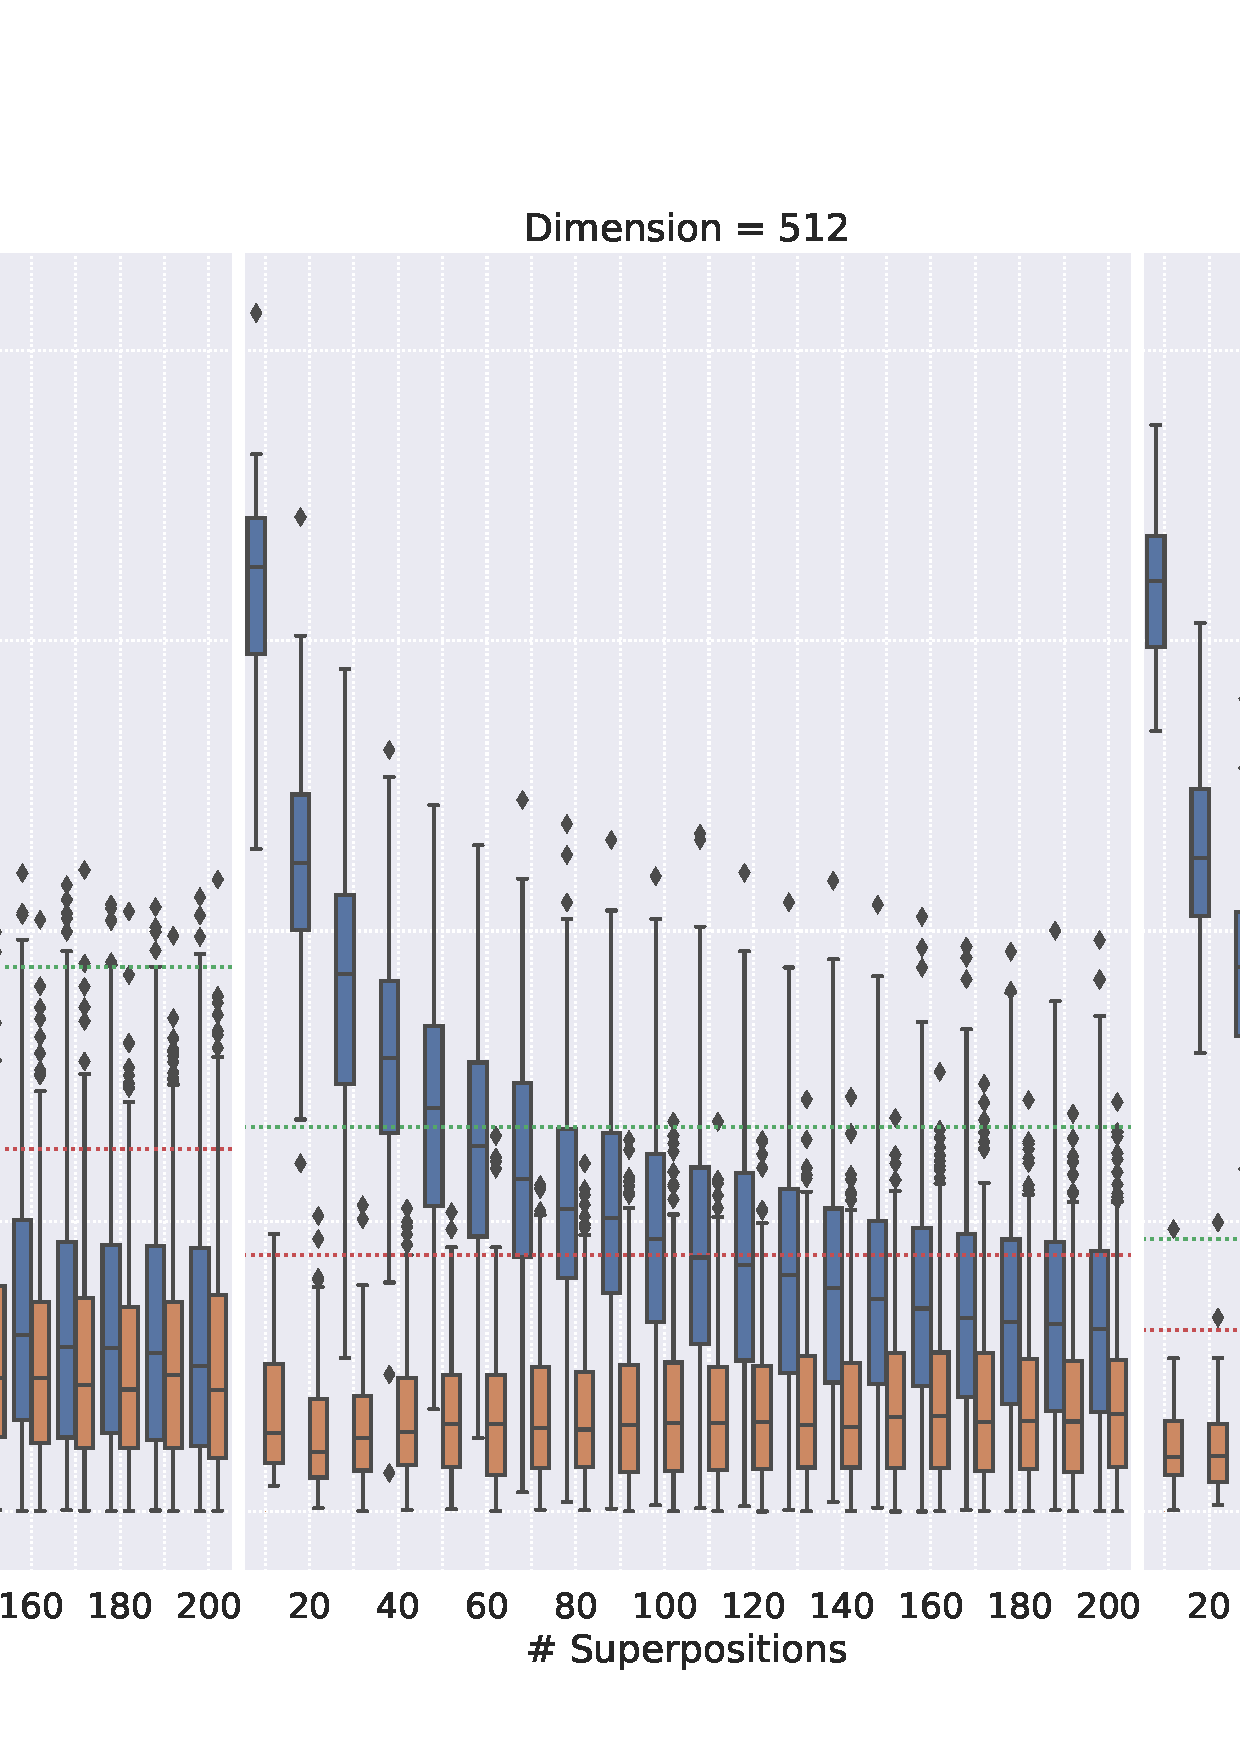
\includegraphics[width=0.95\textwidth]{imgs/spa_superposition_capacity.png}
	\caption{Superposition capacity.}
	\label{fig:spa_superposition_capacity}
\end{figure}

\section{Representational variations}
\subsection{Basic (random) vocabularies}
\subsection{Different vector representations for numerical values}
In this section, we investigate different approaches to map numerical information to semantic vectors.
Therefore, we will focus on
\subsubsection{Scalar multiplication encoding}
\subsubsection{Sine and Cosine encoding with different frequencies and offsets}
For vectorization of two-dimensional values, we use an encoding with sine and cosine functions with different spatial frequencies and offsets.
Therefore, we define the following helper functions
\[ \abb{f_{\left(m,i\right)}}{\mathbb{R}^2}{\mathbb{R}^4}{\left(x,y\right)}{\left(\cos\frac{m\cdot \pi + x}{i + 1}, \sin\frac{m\cdot \pi + x}{i + 1}, \cos\frac{m\cdot \pi + y}{i + 1}, \sin\frac{m\cdot \pi + y}{i + 1}\right)},
\]
\[
\abb{\psi_i}{\mathbb{R}^2}{\mathbb{R}^4}{\left(x,y\right)}{\left(f_{\left(0,i\right)}\left(x,y\right), f_{\left(\frac{1}{2},i\right)}\left(x,y\right), f_{\left(1,i\right)}\left(x,y\right), f_{\left(\frac{3}{2},i\right)}\left(x,y\right)\right)}
\]
and obtain the final vector representation of acceleration in $x$/$y$-direction via the function
\[
\abb{\lambda}{\mathbb{R}^2}{\mathbb{R}^D}{\left(x,y\right)}{\frac{1}{\sqrt{\frac{D}{2}}}\left(\psi_0\left(x,y\right), \cdots, \psi_{\frac{D}{16}-1}\left(x,y\right)\right).}
\]
This encoding $\lambda\left(a_x, a_y\right)$ leads to normalized, nonzero, similar vectors with information distributed over all elements (in contrast to a simple encoding like $\left(a_x, a_y, 0 \cdots, 0\right)$).
\subsubsection{Convolutive power encoding}
\subsection{Encoding visual and semantic structure}
